% !TeX root = ../main.tex

\chapter{个人贡献}

在此次大作业中,我负责使用 C 语言对算法 (\ref{Algorithm:RMFA}) 和算法 (\ref{Algorithm:DFAS}) 进行具体的实现,具体的代码如图 (\ref{Implement}) 所示。在编写这两个算法的实现时,我们通过使用 CMake 进行构建,所使用的 CMakeLists.txt 源码如图 (\ref{CMakeLists}) 所示。

\begin{figure}[htb]
    \centering
    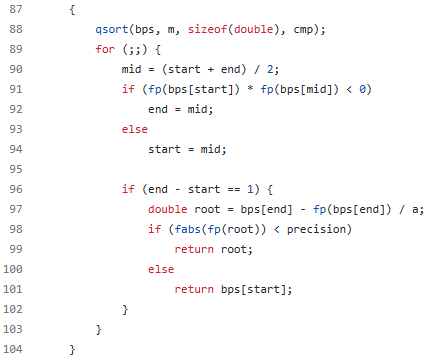
\includegraphics[width=0.45\textwidth]{figures/c@rf_sort().png}
    \qquad
    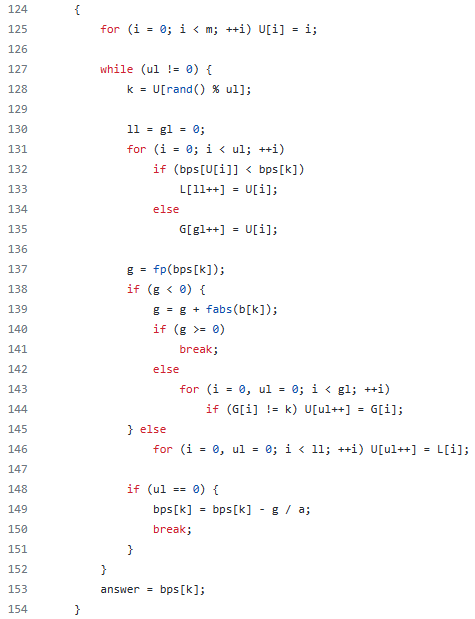
\includegraphics[width=0.45\textwidth]{figures/c@rf_a3().png}
    \caption{算法 (\ref{Algorithm:RMFA})(左) 和算法 (\ref{Algorithm:DFAS})(右) 的具体实现}
    \label{Implement}
\end{figure}

\begin{figure}[htb]
    \centering
    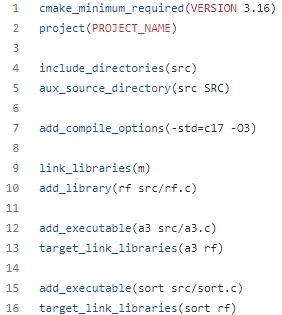
\includegraphics[width=0.5\textwidth]{figures/c@CMakeLists.png}
    \caption{CMakeLists.txt 源码}
    \label{CMakeLists}
\end{figure}

我们通过 cmake 命令进行构建,构建后将会生成 makefile 文件。在生成 makefile 文件后,再次使用 make 命令即可编译出二进制文件,构建的过程如图 (\ref{Build}) 所示。

\begin{figure}[htb]
    \centering
    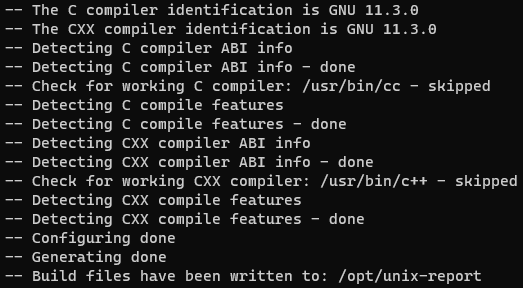
\includegraphics[width=0.45\textwidth]{figures/c@cmake.png}
    \qquad
    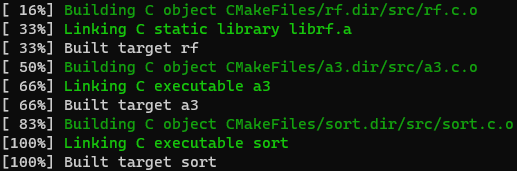
\includegraphics[width=0.45\textwidth]{figures/c@make.png}
    \caption{cmake(左) 与 make(右) 的构建过程}
    \label{Build}
\end{figure}

为了便于组内成员编写测试脚本,我们在程序内设定了计时器。最初版本的计时器仅记录算法的运行时间,而不对内存分配的时间进行记录。然而,这样是难以进行准确的计时,两个算法在较低数据量时的运行时间均较小,无法进行比较。因此,我们将内存分配时间也计入算法的运行时间,这样的记录方法既符合了实际应用中这两种算法的具体运行时间,也使得时间更容易进行记录和对比。图 (\ref{Clock}) 所示的源代码第 8 行、第 15 行便展示了我们记录算法运行时间的过程。

\begin{figure}[htb]
    \centering
    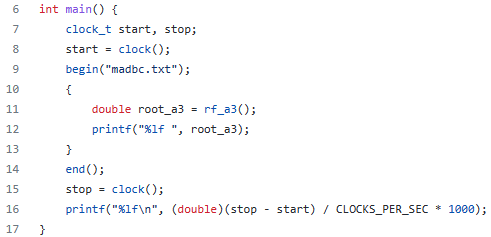
\includegraphics[width=0.5\textwidth]{figures/c@clock}
    \caption{计时相关的源代码}
    \label{Clock}
\end{figure}

图 (\ref{Implement})、图 (\ref{CMakeLists}) 和图 (\ref{Clock}) 中的源代码均已经上传至 GitHub 仓库 \href{https://github.com/xqm32/unix-report}{https://github.com/xqm32/unix-report},仓库中还包含了组内其他成员编写的数据生成脚本和测试脚本。